\documentclass[11pt,letterpaper]{article}
\usepackage[top=3cm, bottom=2cm, left=2cm, right=2cm, columnsep=20pt]{geometry}
\usepackage{pdfpages}
\usepackage{graphicx}
\usepackage{etoolbox}
\apptocmd{\sloppy}{\hbadness 10000\relax}{}{}
% \usepackage[numbers]{natbib}
\usepackage[T1]{fontenc}
\usepackage{ragged2e}
\usepackage[french]{babel}
\usepackage{listings}
\usepackage{color}
\usepackage{soul}
\usepackage[utf8]{inputenc}
\usepackage[export]{adjustbox}
\usepackage{caption}
\usepackage{amsmath}
\usepackage{amssymb}
\usepackage{float}
\usepackage{csquotes}
\usepackage{fancyhdr}
\usepackage{wallpaper}
\usepackage{siunitx}
\usepackage[indent]{parskip}
\usepackage{textcomp}
\usepackage{gensymb}
\usepackage{multirow}
\usepackage[hidelinks]{hyperref}
\usepackage{abstract}
\renewcommand{\abstractnamefont}{\normalfont\bfseries}
\renewcommand{\abstracttextfont}{\normalfont\itshape}
\usepackage{titlesec}
\titleformat{\section}{\large\bfseries}{\thesection}{1em}{}
\titleformat{\subsection}{\normalsize\bfseries}{\thesubsection}{1em}{}
\titleformat{\subsubsection}{\normalsize\bfseries}{\thesubsubsection}{1em}{}

\usepackage{xcolor}
\definecolor{codegreen}{rgb}{0,0.6,0}
\definecolor{codegray}{rgb}{0.5,0.5,0.5}
\definecolor{codepurple}{rgb}{0.58,0,0.82}
\definecolor{backcolour}{rgb}{0.95,0.95,0.92}
\lstdefinestyle{mystyle}{
    backgroundcolor=\color{backcolour},   
    commentstyle=\color{codegreen},
    keywordstyle=\color{magenta},
    numberstyle=\tiny\color{codegray},
    stringstyle=\color{codepurple},
    basicstyle=\ttfamily\footnotesize,
    breakatwhitespace=false,         
    breaklines=true,                 
    captionpos=b,                    
    keepspaces=true,                 
    numbers=left,                    
    numbersep=5pt,                  
    showspaces=false,                
    showstringspaces=false,
    showtabs=false,                  
    tabsize=2
}
\lstset{style=mystyle}

\usepackage[most]{tcolorbox}
\newtcolorbox{note}[1][]{
  enhanced jigsaw,
  borderline west={2pt}{0pt}{black},
  sharp corners,
  boxrule=0pt, 
  fonttitle={\large\bfseries},
  coltitle={black},
  title={Note:\ },
  attach title to upper,
  #1
}

%----------------------------------------------------

\setlength{\parindent}{0pt}
\DeclareCaptionLabelFormat{mycaptionlabel}{#1 #2}
\captionsetup[figure]{labelsep=colon}
\captionsetup{labelformat=mycaptionlabel}
\captionsetup[figure]{name={Figure }}
\newcommand{\inlinecode}{\normalfont\texttt}
\usepackage{enumitem}
\setlist[itemize]{label=\textbullet}

\begin{document}
\begin{titlepage}
\center

\begin{figure}
    \ThisULCornerWallPaper{.4}{Polytechnique_signature-RGB-gauche_FR.png}
\end{figure}
\vspace*{2 cm}

\textsc{\Large \textbf{PHS2223 --} Introduction à l'optique moderne}\\[0.5cm]
\large{\textbf{Équipe : 04}}\\[1.5cm]

\rule{\linewidth}{0.5mm} \\[0.5cm]
\Large{\textbf{Expérience 4}} \\[0.2cm]
\text{Filtrage spatial}\\
\rule{\linewidth}{0.2mm} \\[2.3cm]

\large{\textbf{Présenté à}\\
  Guillaume Sheehy\\
  Esmat Zamani\\[2.5cm]
  \textbf{Par :}\\
  Émile \textbf{Guertin-Picard} (2208363)\\
  Laura-Li \textbf{Gilbert} (2204234)\\
  Tom \textbf{Dessauvages} (2133573)\\[3cm]}

\large{\today\\
Département de Génie Physique\\
Polytechnique Montréal\\}

\end{titlepage}

%----------------------------------------------------

\tableofcontents
\pagenumbering{roman}
\newpage

\pagestyle{fancy}
\setlength{\headheight}{14pt}
\renewcommand{\headrulewidth}{0pt}
\fancyfoot[R]{\thepage}

\pagestyle{fancy}
\fancyhf{}
\renewcommand{\headrulewidth}{1pt}
\fancyhead[L]{\textbf{PHS2223}}
\fancyhead[C]{Rapport préliminaire}
\fancyhead[R]{\today}
\fancyfoot[R]{\thepage}

\pagenumbering{arabic}
\setcounter{page}{1}

%----------------------------------------------------

\section{Introduction}

\section{Théorie}

\subsection{Optique de Fourier}

\subsection{Diffraction et système 4f}

\subsection{Signaux, images et filtres}

\section{Méthodologie}

\subsection{Présentations des montages}

\subsection{Explications}

\section{Hypothèses}

Afin de mieux comprendre et prédire ce qui sera vu avec les montages présentés précédemment, il est possible d'émettre quelques hypothèses en lien avec l'application de filtres sur des images. Cette section présente donc le filtrage et l'analyse d'images de référence disponible dans le répertoire du cours.

\subsection{Patron d'échec}

La première image filtrée est un simple patron d'échec. Pour appliquer un filtre, la transformée de Fourier de l'image est prise, tel qu'affiché à la figure \ref{echec_patron} :

\begin{figure}[H]
  \centering
  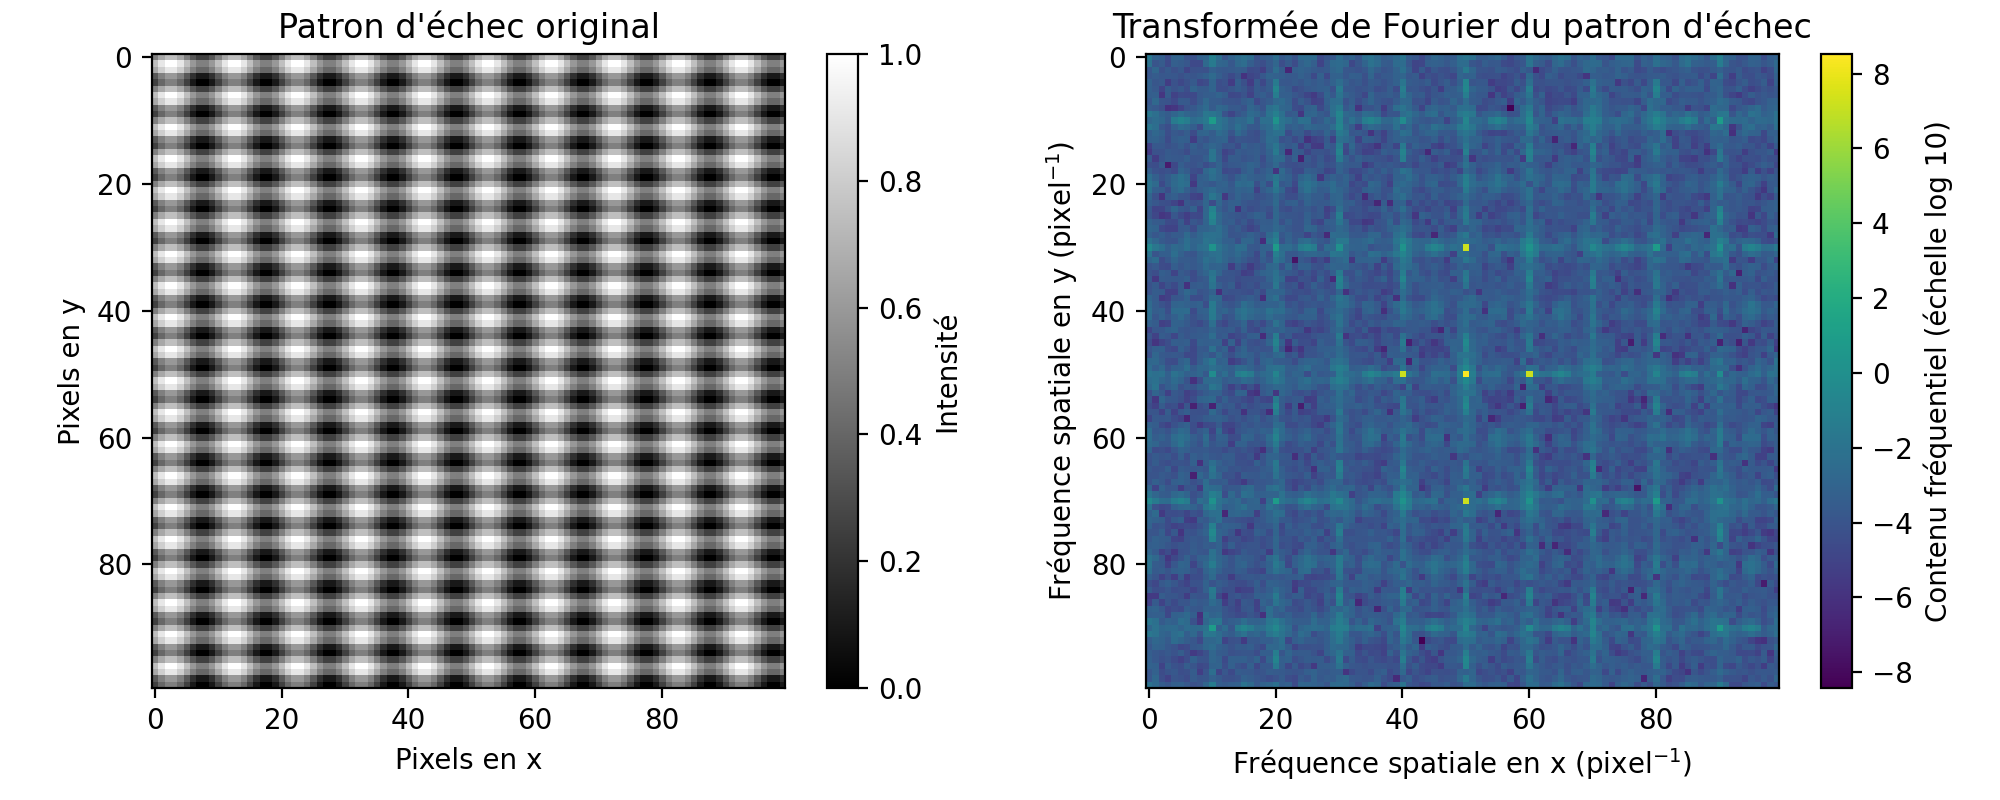
\includegraphics[scale=0.68]{check.png}
  \caption{Affichage du patron d'échec original et de sa transformée de fourier}
  \label{echec_patron}
\end{figure}

Pour enlever les oscillations en $\hat{y}$, la fonction fenêtre de la figure \ref{echec_filtre}, qui agit comme filtre passe-bande, est appliquée sur la transformée de Fourier :

\begin{figure}[H]
  \centering
  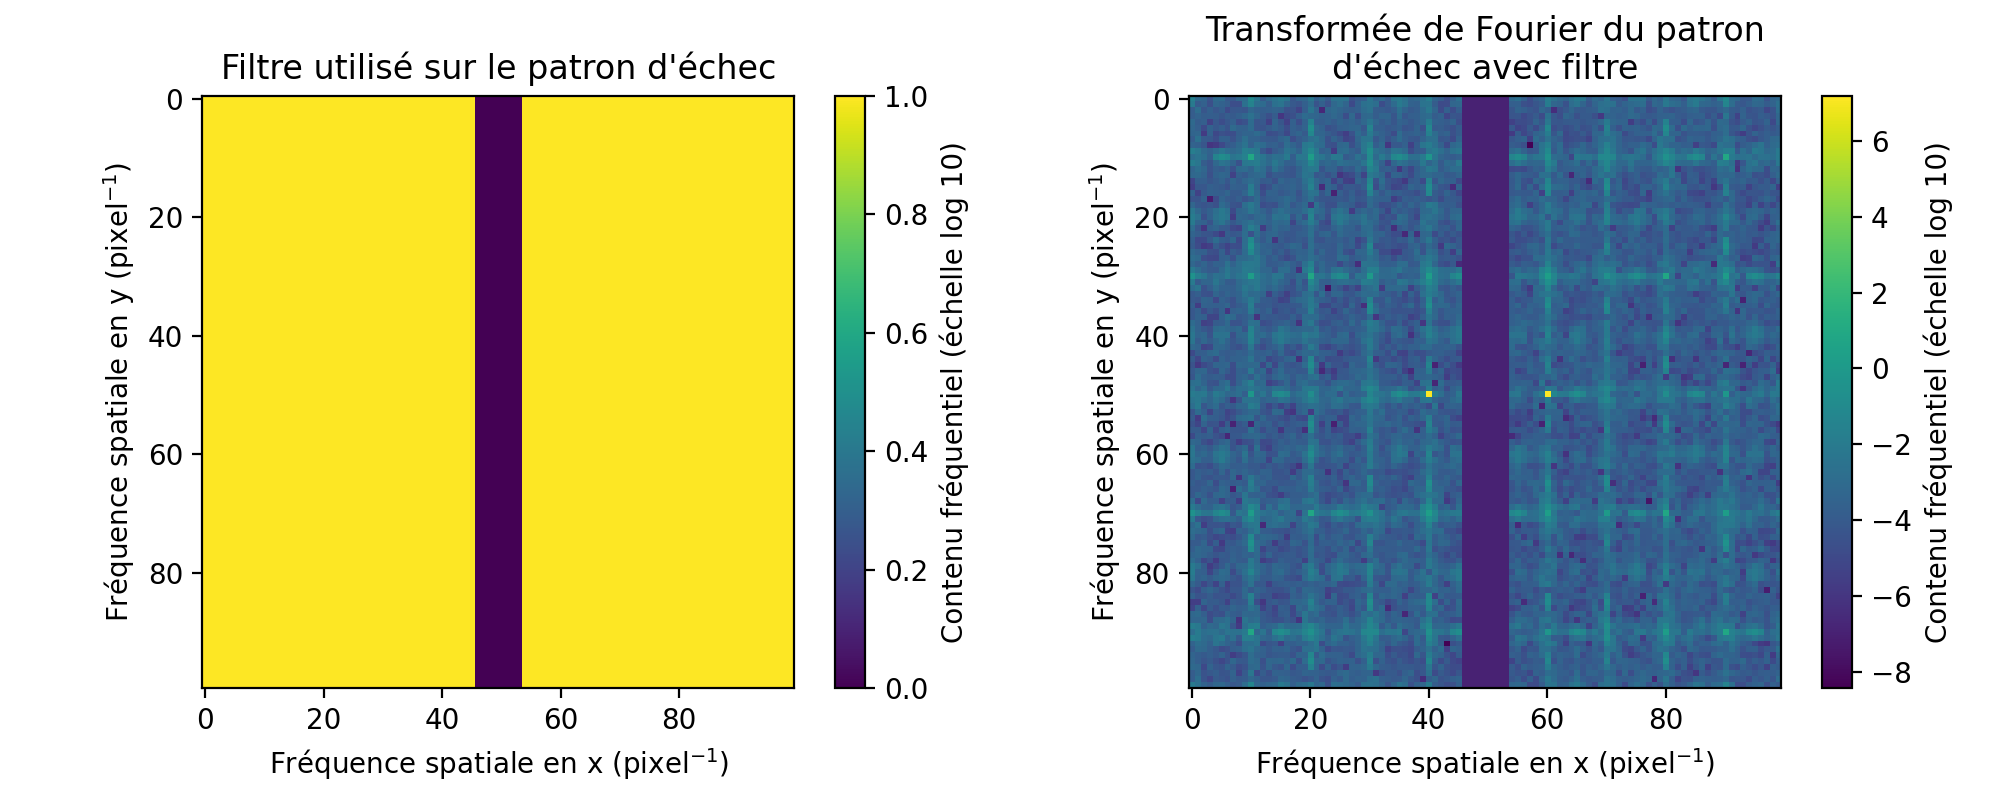
\includegraphics[scale=0.68]{check_mask.png}
  \caption{Filtre utilisé pour enlever les oscillations en $\hat{y}$ et son applications sur la transformée de Fourier}
  \label{echec_filtre}
\end{figure}

Enfin, la transformée inverse sur l'application du filtre donne le patron d'échec avec toutes les orcillations en $\hat{y}$ filtrées, tel que montré à la figure \ref{echec_comp} :

\begin{figure}[H]
  \centering
  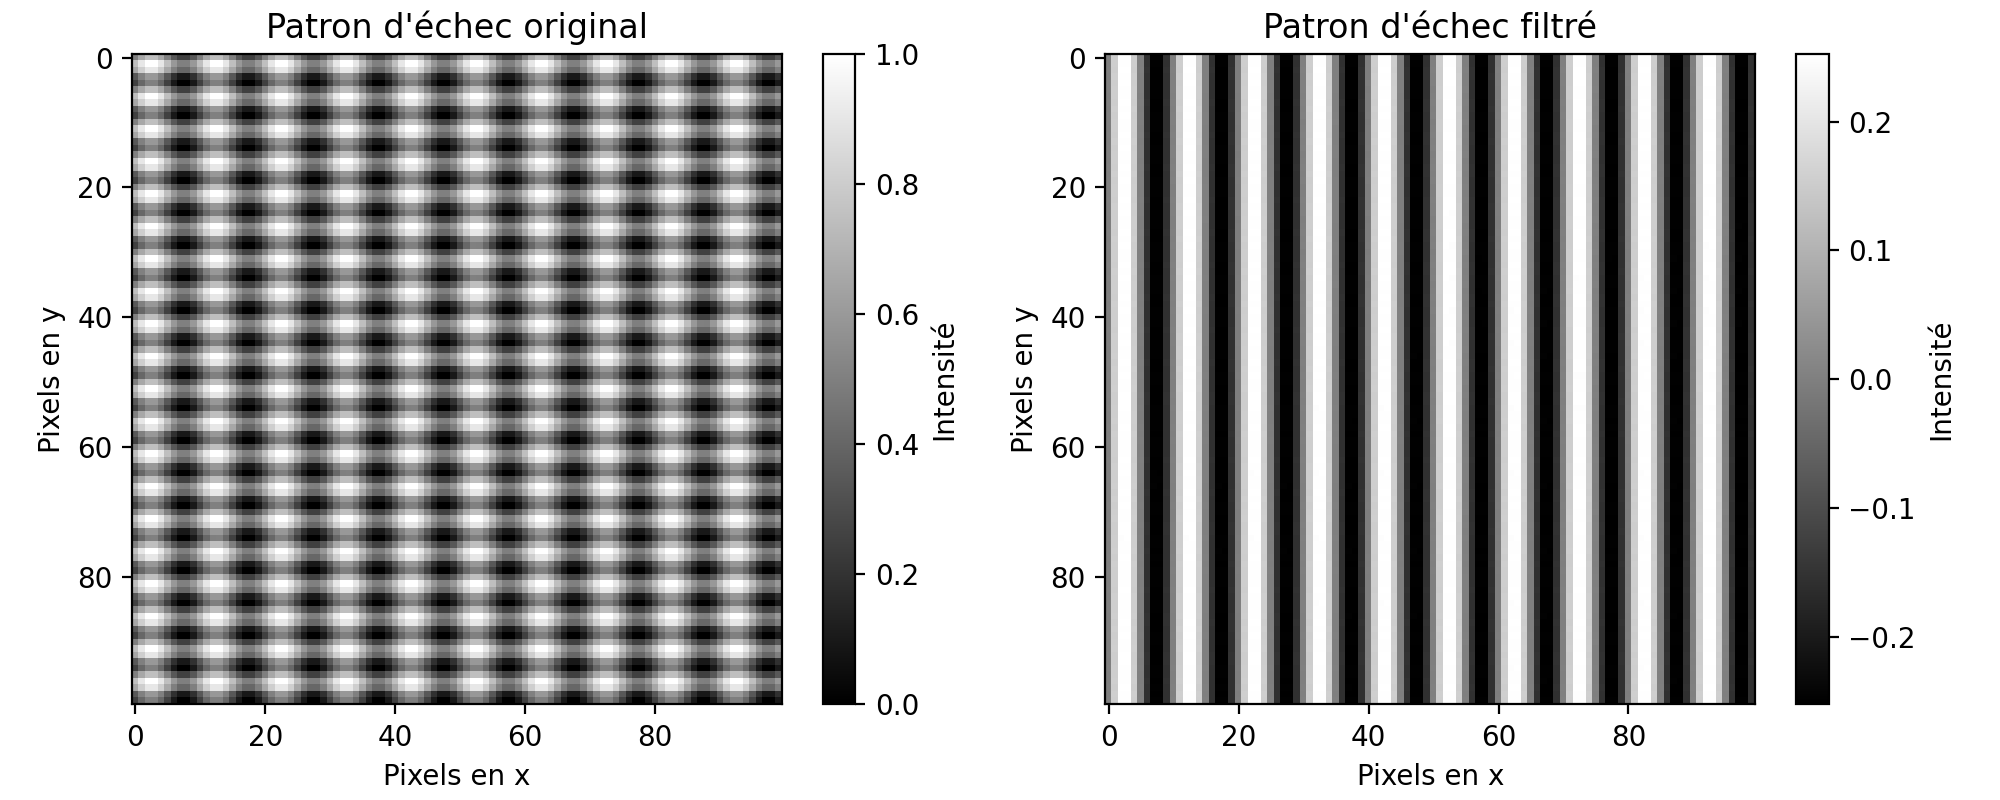
\includegraphics[scale=0.68]{check_filtre.png}
  \caption{Comparaison entre le patron d'échec initial et filtré}
  \label{echec_comp}
\end{figure}

\subsection{Filtres passe-bas top-hat}

La seconde image filtrée est celle du chat Marvin. Il est possible de la voir ainsi que sa transformée de Fourier à la figure \ref{cat_og}. Ensuite, des filtre passe-bas top hat sont défini aussi comme des fenêtres mais circulaires. Il est possible de voir ces filtres et leurs applications aux figures \ref{fc50hat}, \ref{fc75} et \ref{fc100} pour $f_c = 50, 75,100$ respectivement.

\begin{figure}[H]
  \centering
  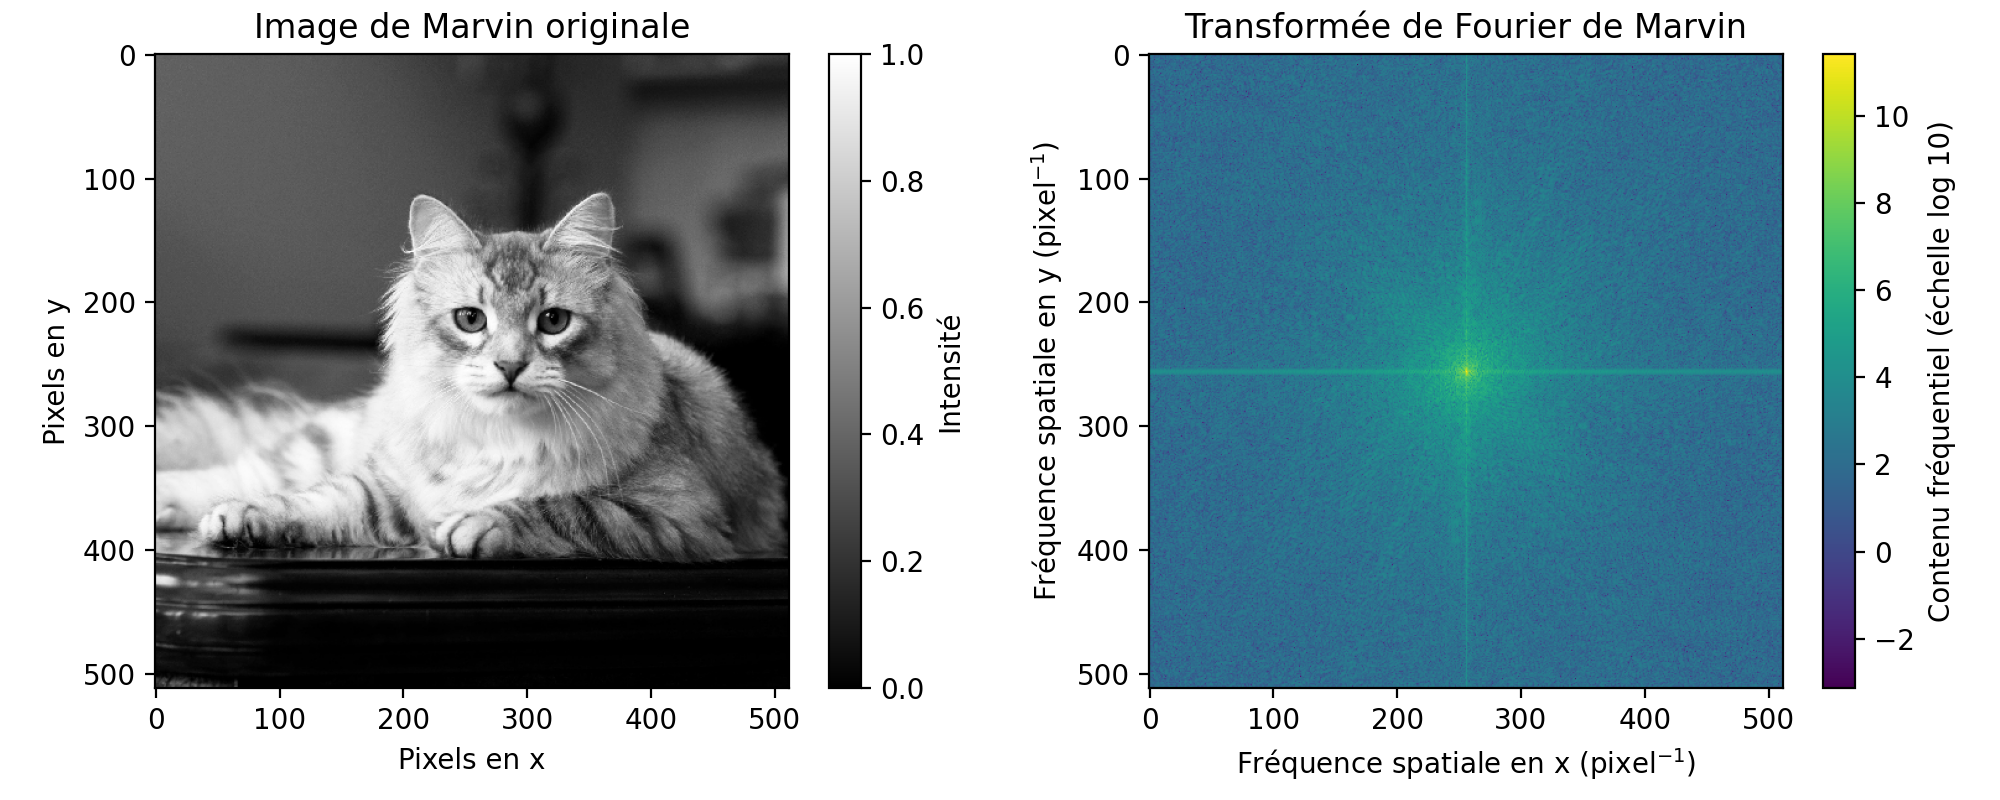
\includegraphics[scale=0.68]{marvin_og.png}
  \caption{Image originale de Marvin et de sa transformée de Fourier}
  \label{cat_og}
\end{figure}

\begin{figure}[H]
  \centering
  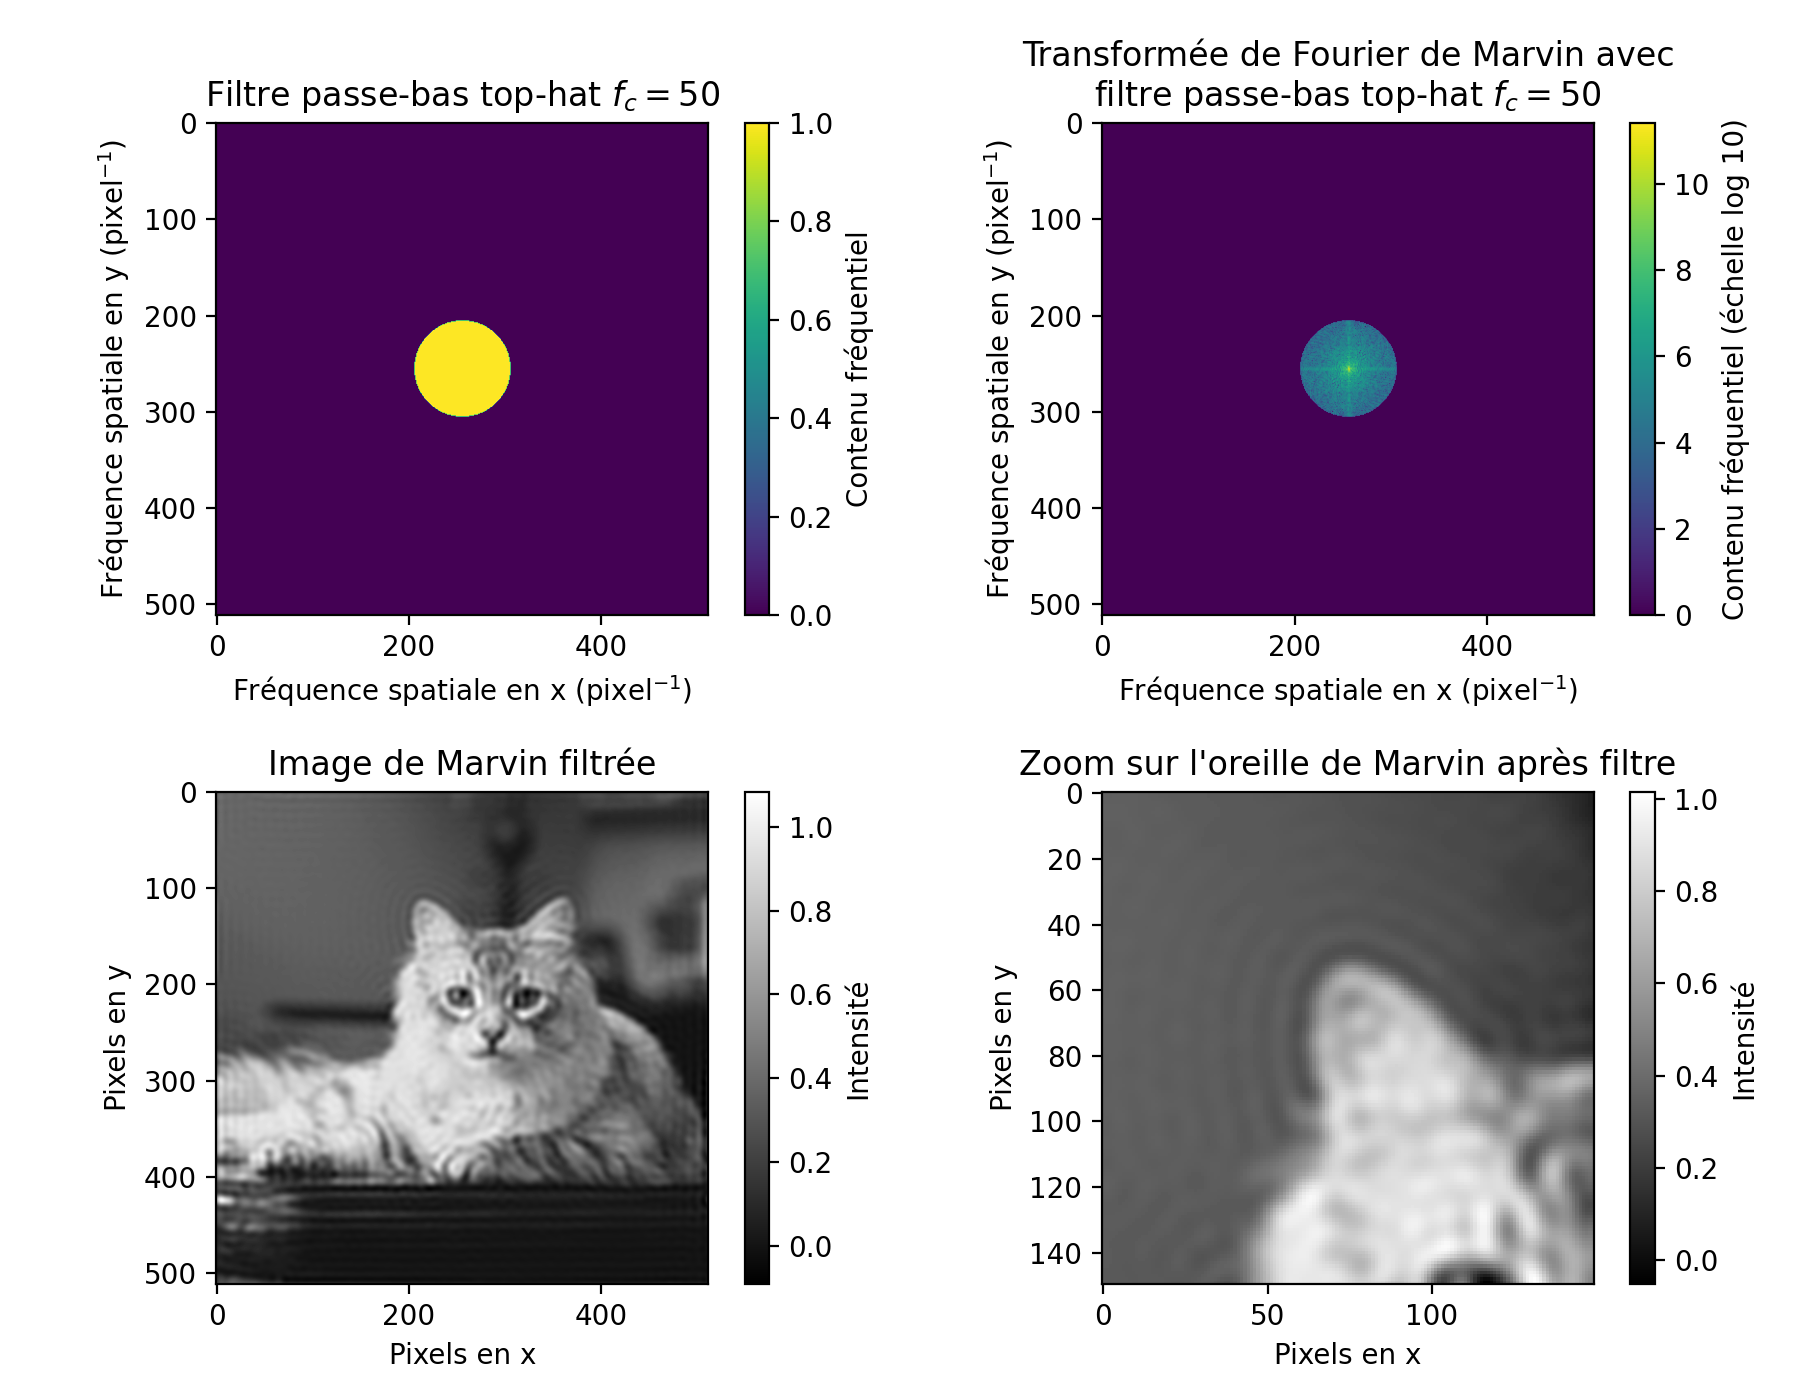
\includegraphics[scale=0.7]{marvin_post_filter_fc_50.png}
  \caption{Filtre passe-bas top-hat à $f_c = 50$ pixels$^{-1}$ appliqué sur l'image de Marvin}
  \label{fc50hat}
\end{figure}

\begin{figure}[H]
  \centering
  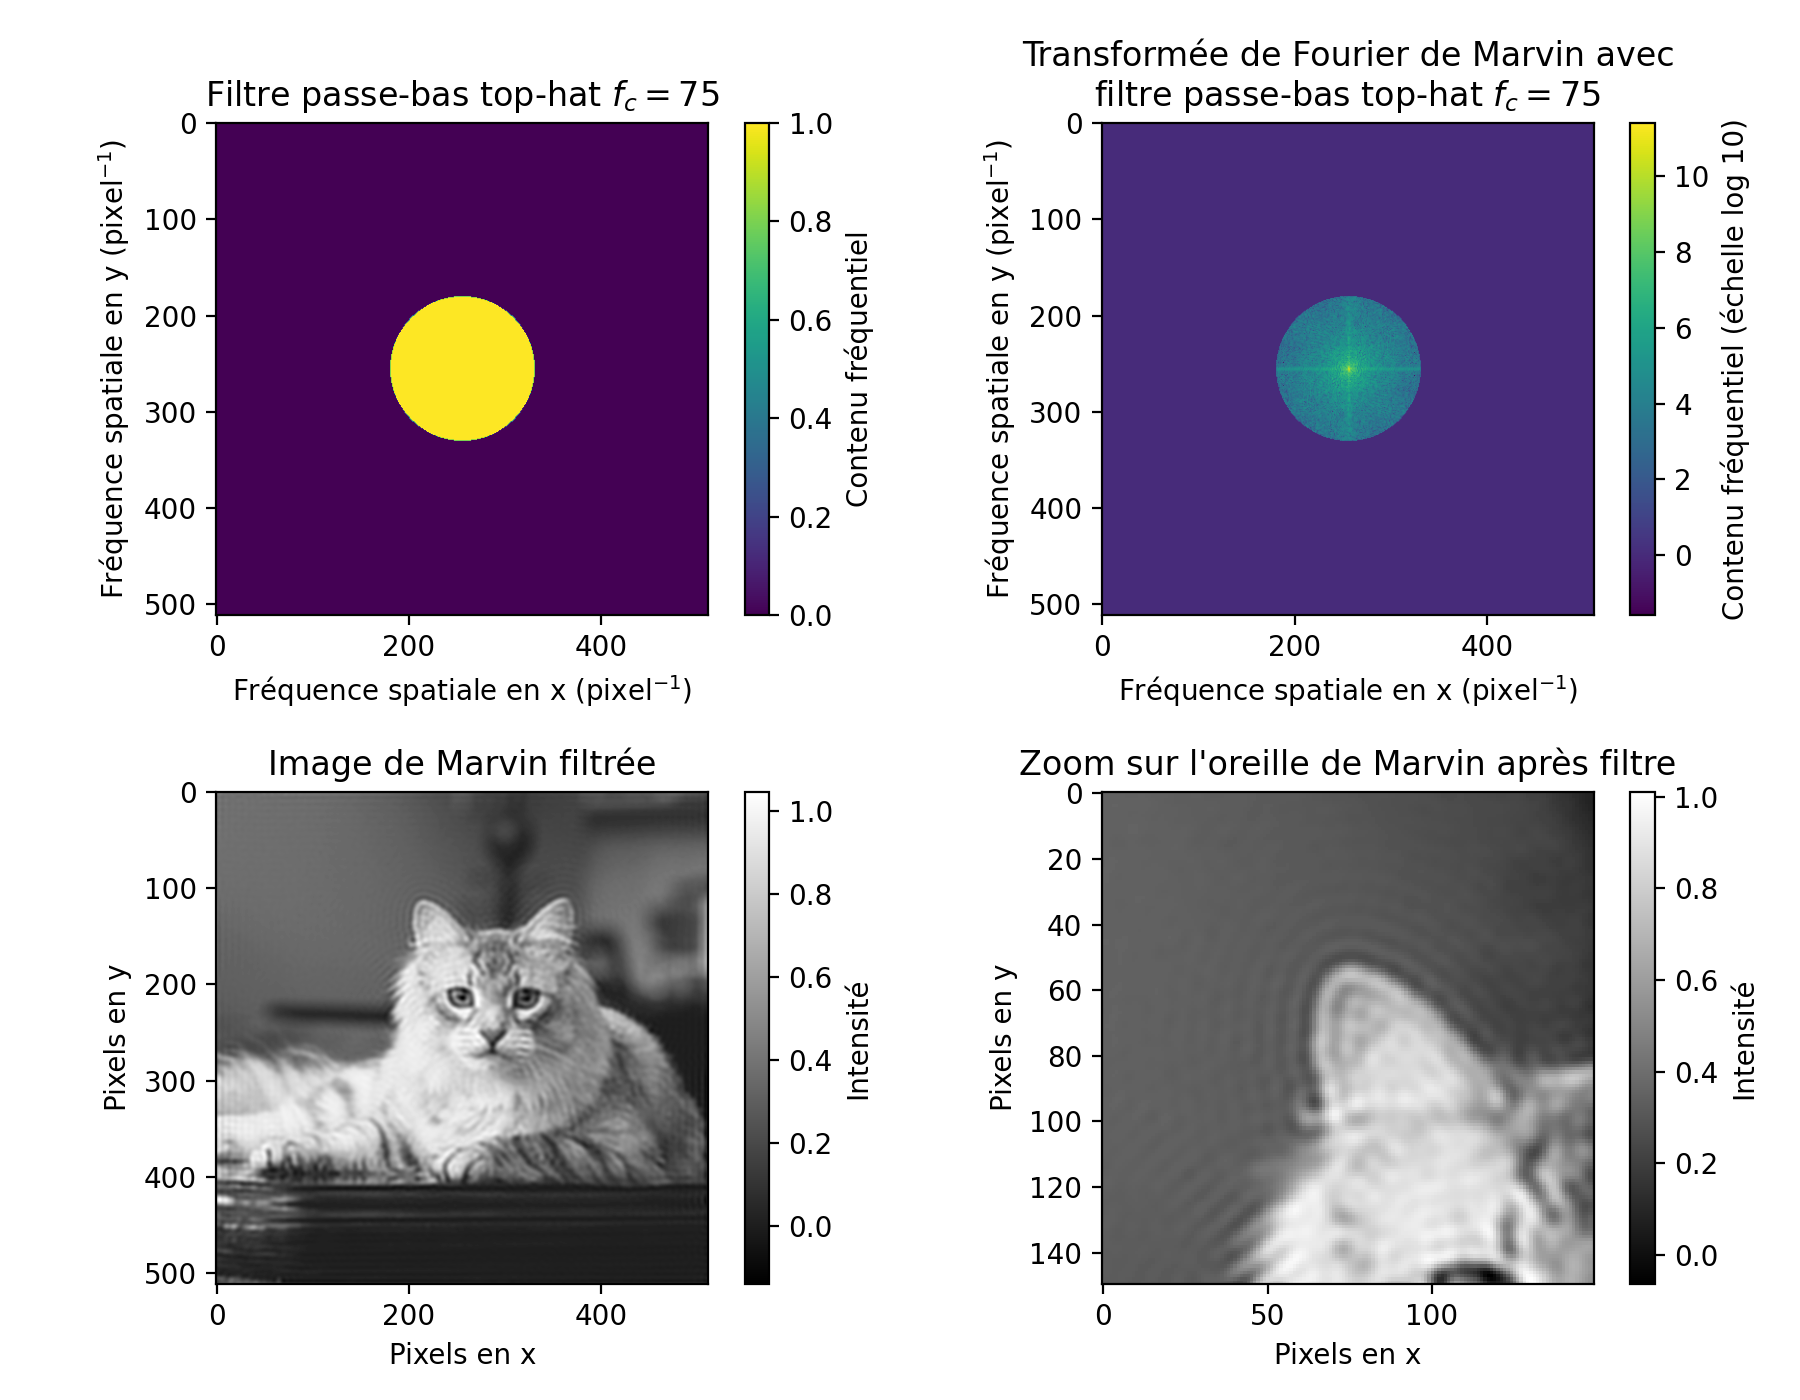
\includegraphics[scale=0.7]{marvin_post_filter_fc_75.png}
  \caption{Filtre passe-bas top-hat à $f_c = 75$ pixels$^{-1}$ appliqué sur l'image de Marvin}
  \label{fc75}
\end{figure}

\begin{figure}[H]
  \centering
  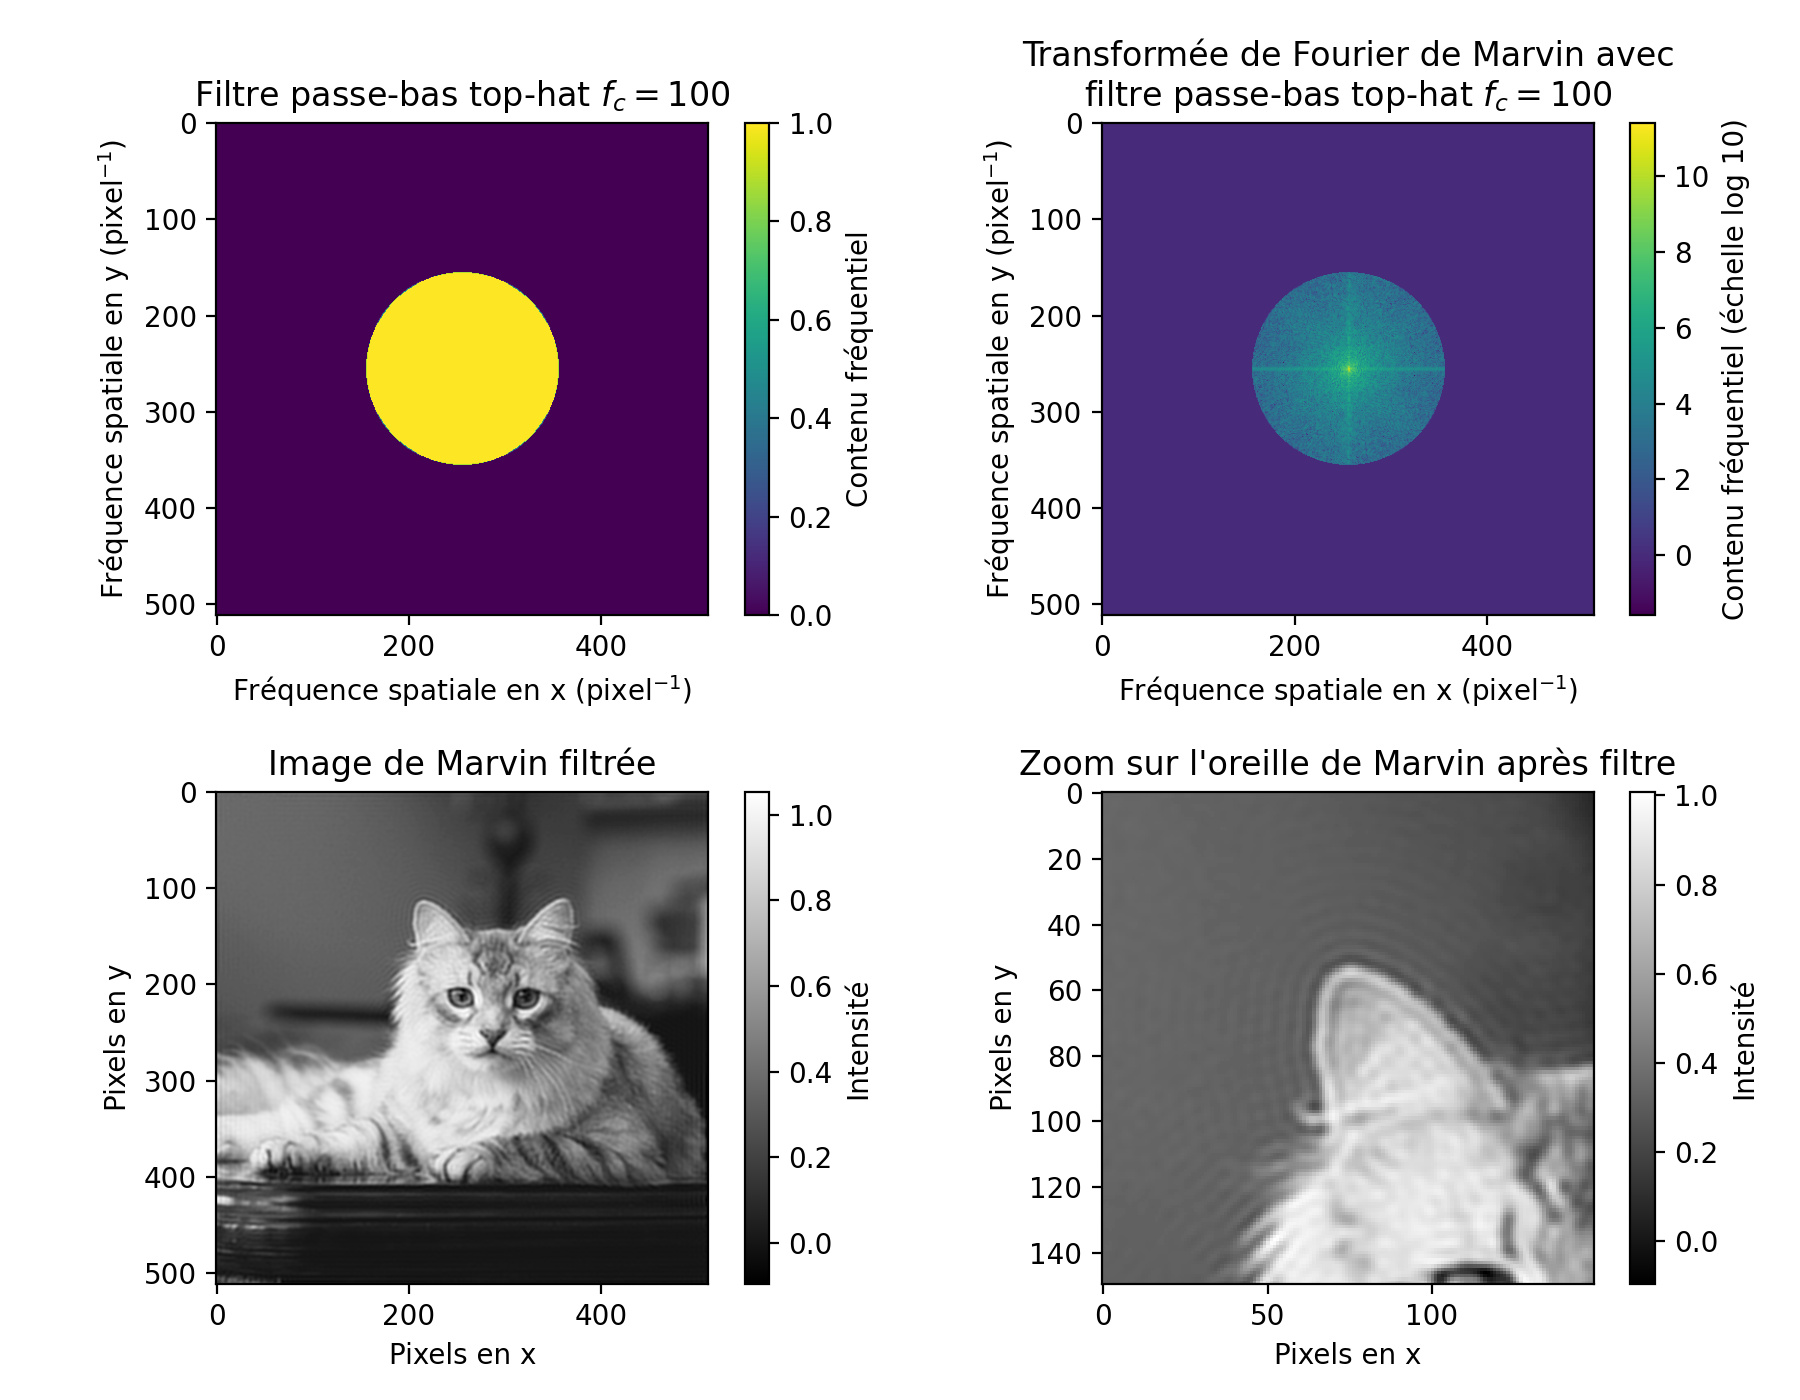
\includegraphics[scale=0.7]{marvin_post_filter_fc_100.png}
  \caption{Filtre passe-bas top-hat à $f_c = 100$ pixels$^{-1}$ appliqué sur l'image de Marvin}
  \label{fc100}
\end{figure}

Pour les trois figures précédentes, un zoom est aussi fait sur l'oreille gauche de Marvin. Il est possible d'y observer une sorte d'onde qui fait le contour de l'oreille et du reste de la tête. Cet effet est plus prononcé pour les filtres de plus basse fréquence. Cela fait en sorte que l'image filtrée la plus claire est celle avec la fréquence de coupure la plus haute, soit $f_c=100$ pixels$^{-1}$ à la figure \ref{fc100}. Il est donc possible d'émettre l'hypothèse que lors des manipulations, la qualité de l'image filtrée augmentera avec l'ouverture de l'iris, qui va agir comme  le filtre passe-bas top hat ici. L'effet ondulatoire sera discuté plus loin.

\subsection{Filtre gaussien}

Enfin, la figure \ref{gauss} montre l'application d'un filtre gaussien, où la fréquence de coupure $f_c = 50$ pixels$^{-1}$ est défini comme l'écart-type de cette gaussienne :

\begin{equation}
  f(x) = e^{\frac{-\left( x-\mu \right)^{2}}{2f_c^2}}
\end{equation}

où $\mu$ est la position au centre de l'image. Cela donne :

\begin{figure}[H]
  \centering
  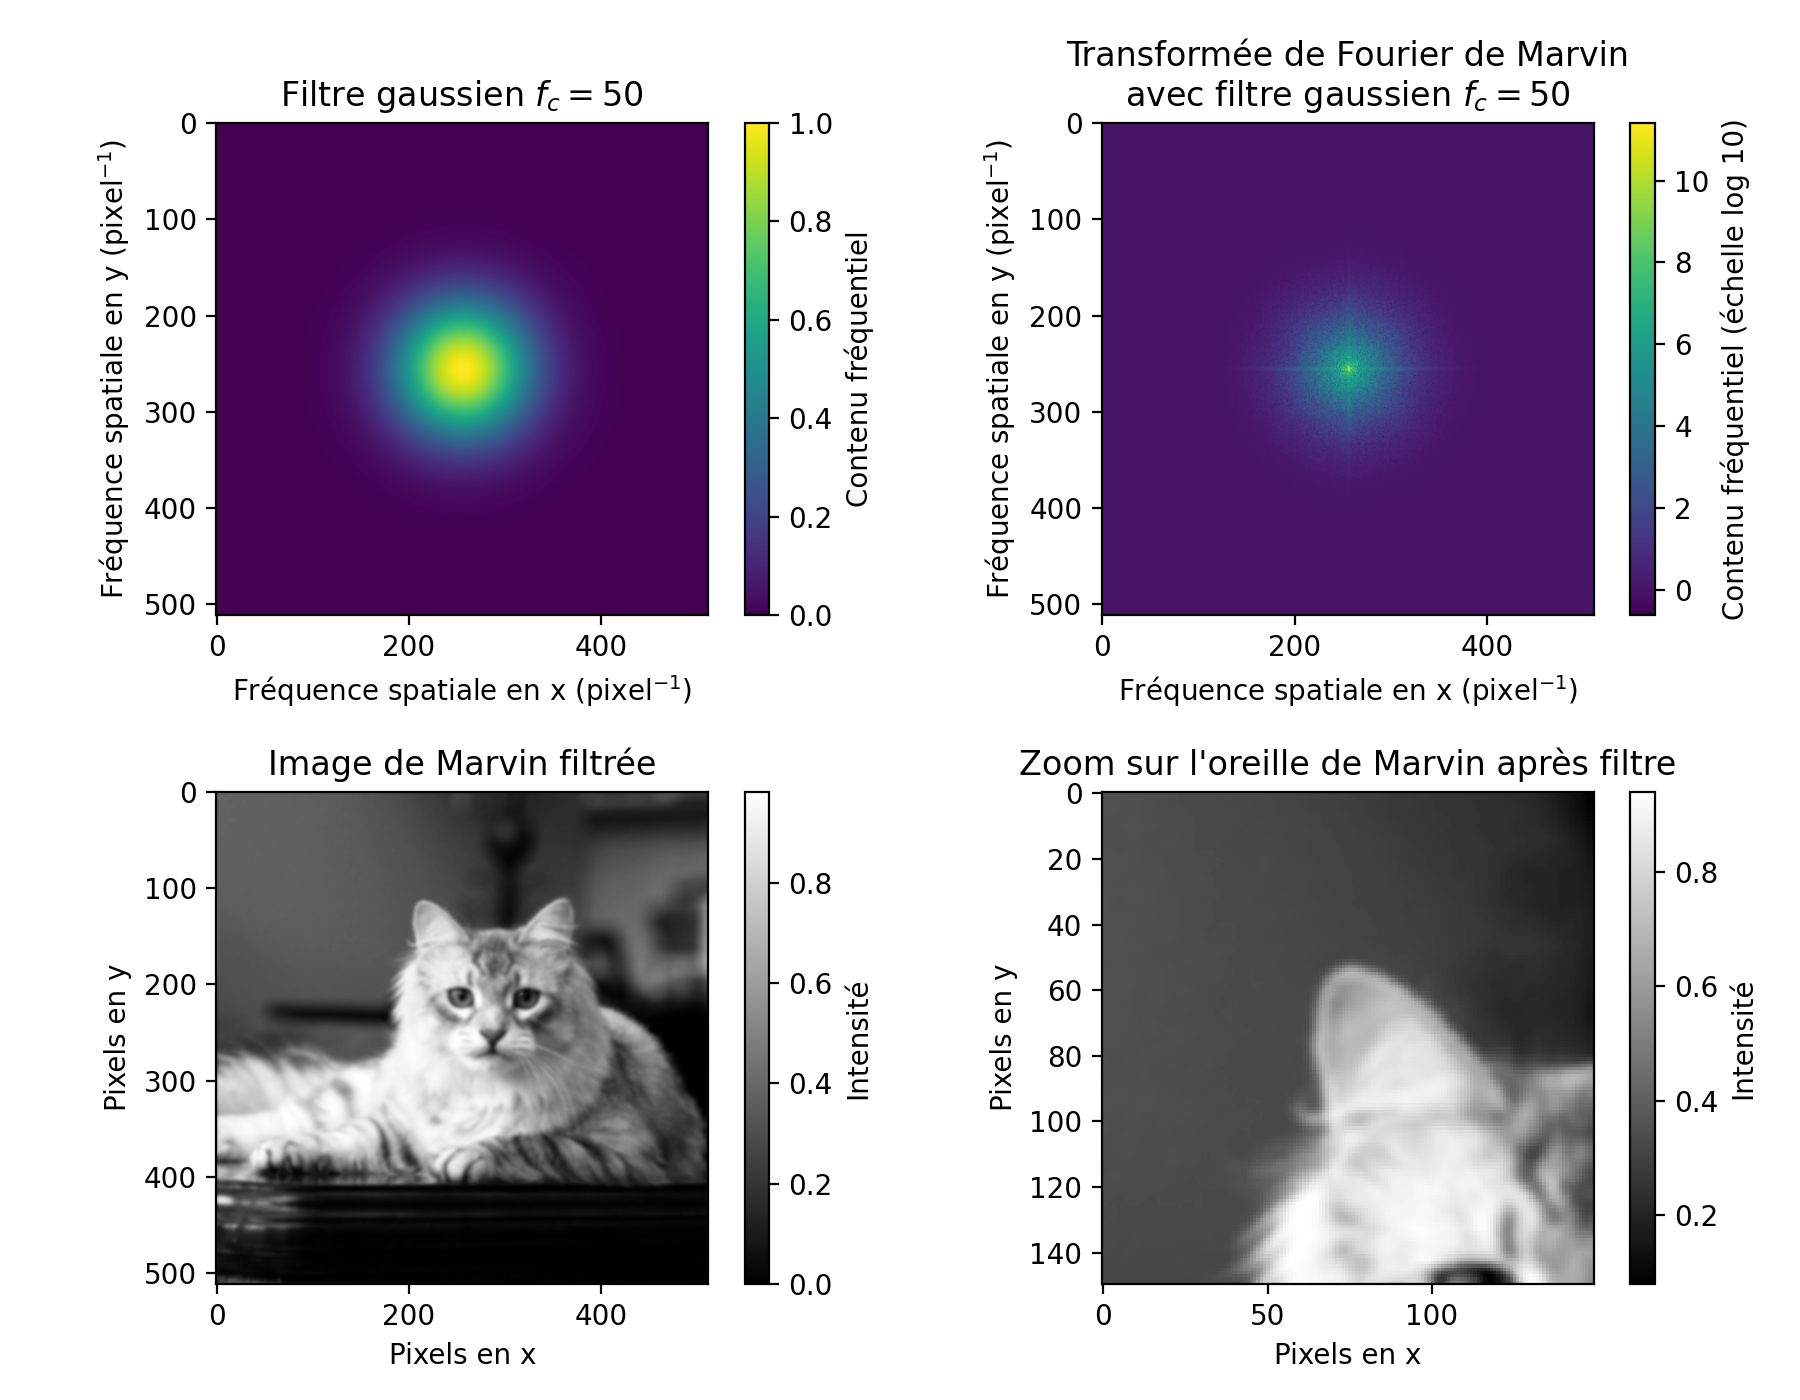
\includegraphics[scale=0.7]{marvin_gauss_fc_50.png}
  \caption{Filtre gaussien à $f_c = 50$ pixels$^{-1}$ appliqué sur l'image de Marvin}
  \label{gauss}
\end{figure}

Le résultat est une image très peu floutée, et en regardant le zoom sur l'oreille, les ondes sont disparues. Le filtre gaussien est donc idéal pour ce cas. Pour expliquer pourquoi le filtre gaussien ne présente pas les ondes, il est bon de se pencher à nouveau sur le filtre top-hat. Ce dernier est essentiellement une fonction rectangle. Sa transformée de fourier est connue comme étant une fonction sinc :

\begin{figure}[H]
  \centering
  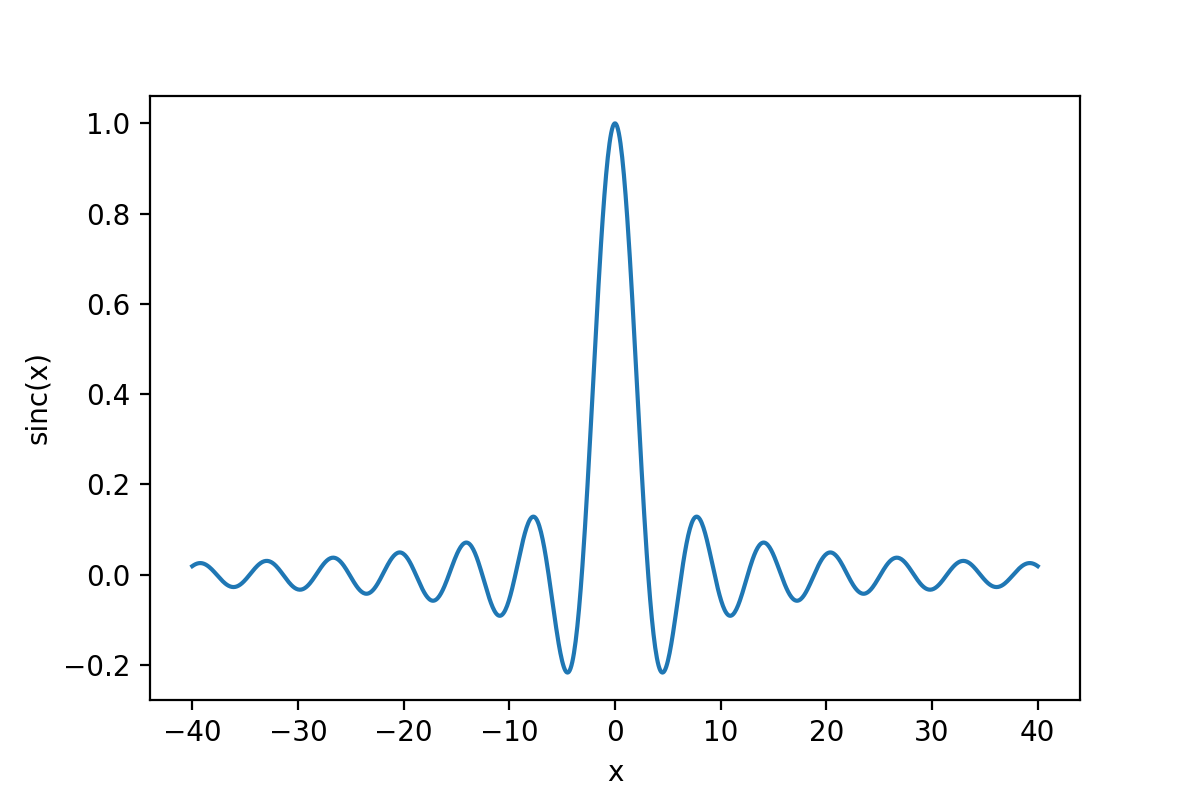
\includegraphics[scale=0.7]{sinc.png}
  \caption{Représentation de la fonction sinc}
  \label{sinc}
\end{figure}

Les ondes observées près des contours sont donc un symptôme de la transformée de Fourier inverse de la fonction rectangle, qui est aussi un sinus cardinal. Les changements drastiques d'intensité voient donc les propriétés du sinc apparaître, notamment les oscillations autour de $\frac{\sin\left( x \right)}{x}  = 0$ pour $x$ éloigné de 0 à la figure \ref{sinc}. C'est l'origine des "ondes" bien visibles près des oreilles de Marvin aux figures \ref{fc50hat}, \ref{fc75} et \ref{fc100}. Quant au filtre gaussien, étant donné qu'une fonction gaussienne est lisse et que sa transformée de Fourier est connue comme étant une autre gaussienne, aucun changement "drastique" ni d'apparence ondulatoire n'est perceptible après le filtrage.

\clearpage

% \bibliographystyle{unsrtnat}
% \bibliography{My_Library}

\end{document}
